%%%%%%%%%%%%%%%%%%%%%%%%%%%%%%%%%%%%%%%%%
% Modern Presentation
% LaTeX Template
% Version 1.0 (02/04/18)
%
% This Template was created by:
% Christoph Becker
%
%%%%%%%%%%%%%%%%%%%%%%%%%%%%%%%%%%%%%%%%%

%----------------------------------------------------------------------------------------
%	PACKAGES AND OTHER DOCUMENT CONFIGURATIONS
%----------------------------------------------------------------------------------------

\documentclass{fancyslides}

\usepackage[utf8]{inputenc} % Allows the usage of non-english characters
\usepackage{times} % Use the Times font
\usepackage{booktabs} % Allows the use of \toprule, \midrule and \bottomrule in tables
\graphicspath{{images/}} % Location of the slide background and figure files
\usepackage{amsmath}
\usepackage{amssymb} % Advanced math symbols
%\usepackage{bm} % Bold math symbols, including upright Greek
\usepackage{euscript}
\usepackage[overload]{textcase} % Overwrite \MakeUppercase with \MakeTextUppercase
\usepackage{textcomp}
\usepackage{multicol}
\usepackage{multirow}
\usepackage{graphicx} % for figures
\usepackage{colortbl}
\usepackage{subcaption}
\usepackage[tocflat]{tocstyle} % Edit Table of Content settings
%\usepackage[T1]{fontenc}
%\usepackage[utf8]{inputenc}
%\renewcommand{\ttdefault}{lcmtt}

%------------------------------------------------
% COLORS
% The following colors are predefined in this class:
%		 white, black, gray, blue, green and orange

% Define your own color as follows:
% Opacity (transparency) for the structure elements (boxes and circles)
\newcommand{\structureopacity}{0.75}
% Set the color of structure elements (boxes and circles)
\definecolor{darkred}{RGB}{153,0,0}
\definecolor{skyblue}{RGB}{102,178,255}
\definecolor{sftorange}{RGB}{255,161,102}
\definecolor{grey}{RGB}{96,96,96}
\definecolor{ltgrey}{RGB}{180,180,180}
\newcommand{\strcolorbkg}{skyblue} % Set color of transparent elements
\newcommand{\strcolortitle}{darkred} % Set color of transparent elements for title page
\newcommand{\gencol}{black} % Set general text color
\newcommand{\strcolortxt}{white} % Set text color on transparent elements
\newcommand{\subtitlecolor}{grey} % Set text color on transparent elements
\newcommand{\vrulecolor}{\color{ltgrey}\vline}
\newcommand{\hlinecolor}{\arrayrulecolor{ltgrey}\hline}

\setlength{\columnseprule}{1pt}
\renewcommand{\columnseprulecolor}{\color{red}}
%------------------------------------------------
% FONT
\newenvironment{typewriter}{\ttfamily}{\par}
\newcommand{\rulesep}{\unskip\ \vrule\ }
\DeclareSymbolFont{euleroperators}{U}{eur}{m}{n}
\SetSymbolFont{euleroperators}{bold}{U}{eur}{b}{n}
\makeatletter
\renewcommand{\operator@font}{\mathgroup\symeuleroperators}
\makeatother

%------------------------------------------------
% Define Font paremeters for sections
% Beamer options - do not change
\usetheme{default}
% Disable the slide navigation buttons on the bottom of each slide
\setbeamertemplate{navigation symbols}{}
\setbeamertemplate{footline}[frame number]
\setbeamercolor{footline}{fg=black}
\setbeamerfont{footline}{family=\fontfamily{qcr}\selectfont,size=\footnotesize}
% Define the color of titles and fixed text elements (e.g. bullet points)
\setbeamercolor{structure}{fg=\gencol}
\setbeamercolor{normal text}{fg=\gencol} % Define the color of text in the presentation
\setbeamercolor{section in toc}{fg=sftorange}
\setbeamerfont{section in toc}{family=\fontfamily{qcr}\selectfont}
\setbeamerfont{section number projected}{size=\Large}
\setbeamercolor{section number projected}{fg=sftorange}
\usefonttheme[onlymath]{serif} % set font for math equations

%----------------------------------------------------------------------------------------
%	Sections/TableOfContent

\AtBeginSection[]{
	\fbckg{smile_cluster.jpg}
	\begin{frame}[plain,noframenumbering]
		\ftitle{Content}
		\begin{typewriter}
		\begin{mybox}
			\large{\textbf{{\color{white}
			\tableofcontents[currentsection]
			}}}
		\end{mybox}
		\end{typewriter}
	\end{frame}
}

%----------------------------------------------------------------------------------------
%	TITLE SLIDE
% Presentation title
\newcommand{\titlephrase}{
\LARGE{\textbf{\texttt{{\color{white}
A Modern PowerPoint \\
\hspace{-1em} Template}}}}}
\newcommand{\name}{\small{John Smith}} % Presenter's name
\newcommand{\affil}{\small{The Willy Wonka Candy Company}} % Presenter's institution
\newcommand{\email}{\small{johnsmith@willywanker.com}} % Presenter's email address

\begin{document}

\startingslidetwo % This command inserts the title slide as the first slide

%----------------------------------------------------------------------------------------
%	PRESENTATION SLIDES
%----------------------------------------------------------------------------------------
% Content ------------------------------------------------
\fbckg{smile_cluster.jpg}
\begin{frame}[plain,noframenumbering]
	\ftitle{Content}
	\begin{typewriter}
	\begin{mybox}
		\large{\textbf{{\color{white}
		\tableofcontents
		}}}
	\end{mybox}
	\begin{textblock}{30}(9.5,15.5)
		{\color{white}\tiny{\texttt{Image Credit: NASA/ESA; HST (WFPC2,WFC3)}}}
	\end{textblock}
	\end{typewriter}
\end{frame}

% Lists ------------------------------------------------
\section{Lists}

\fbckg{white.jpg} % Slide background image
\begin{frame}
	\begin{typewriter}
	\ftitle{How lists look like...} % Convey Message/The 'So-What'
	\begin{itemize} % no more than 6 items ungrouped
		% https://arxiv.org/pdf/1802.02165.pdf
		\item globular properties sensitive to cosmology
		\item their formation from cosmic density field is known
		% https://journals.aps.org/prd/pdf/10.1103/PhysRevD.83.063503
		\item observational measurements have advanced signigicantly
		\item test ground for nonlinear interactions of modified gravity theories with matter
		\item place strongest constraints on $f(R)$ gravity on cosmological scales
	\end{itemize}
	\end{typewriter}
\end{frame}

% Equations ------------------------------------------------
\section{Equations}

\fbckg{white.jpg} % Slide background image
\begin{frame}
	\begin{typewriter}
	\ftitle{...or equations...} % Convey Message/The 'So-What'
	\vspace{4em}
	\begin{itemize} % no more than 6 items ungrouped
		%\setlength\itemsep{2em}
		% https://arxiv.org/pdf/1802.02165.pdf
		\item modified Einstein-Hilbert action\\
			\begin{equation*}
				S=\int d^{4}x\sqrt{-g} \Big[\frac{R + {\color{red}f(R)}}{16\pi G} \Big]
			\end{equation*}
		%\item extra scalar d.o.f. $f_{R} \equiv df/dR$
		\item modified Einstein equation\\
			\begin{equation*}
				G_{\mu\nu} {\color{red}+ X_{\mu\nu}} = 8\pi G T_{\mu\nu}
			\end{equation*}
		\item modified Poisson equation\\
			\begin{equation*}
				\nabla^{2}\Phi = {\color{red}\frac{4}{3}}4\pi G\delta\rho {\color{red}- \frac{1}{6}\delta R}
			\end{equation*}
		% https://journals.aps.org/prd/pdf/10.1103/PhysRevD.83.063503
		%\item physical range of scalaron defined by Compton wavelength
		%	$\lambda_{C} = a^{-1}\Big(3f_{RR}\Big)^{1/2}$
		%\item converges to GR in deep potential wells (chameleon screening)
	\end{itemize}
	\end{typewriter}
\end{frame}

% Data ------------------------------------------------
\section{Tables}
% https://arxiv.org/pdf/1205.3984.pdf :
% BAO, WL, SNIa the Gaussian nature of the likelihood functions is less explored than in the case of CMB anisotropis

\fbckg{white.jpg} % Slide background image
\begin{frame}
	\begin{typewriter}
	\ftitle{...or tables...}
%	\hspace*{-8pt}\makebox[\linewidth][c]{%
	\begin{table}
		\label{tab:data}
		\begin{tabular}{p{1.8cm} !{\vrulecolor} p{2cm} p{1.6cm} !{\vrulecolor} p{2.25cm} p{1.6cm}}
			& {\color{red}Cataneo} & & {\color{red}Mak} & \\ \hlinecolor
			{\color{blue}Clusters} & \small{$224$,\newline $z<0.5$,\newline $M_{\text{true}}$} & \small{ROSAT} &
			\small{$\sim 3000$,\newline $0.15<z$,\newline $M_{vir}>10^{14}M_{\odot}$} & \small{Planck, SPT, SPTpol, ACTpol} \\ \hlinecolor
			{\color{blue}CMB} & \small{$z\sim1100$}& \small{WMAP, Planck, ACT, SPT} & \small{$z\sim1100$} & \small{Planck} \\ \hlinecolor
			{\color{blue}SNIa} & \small{$580$, \newline $z<1.5$} & \small{Union 2.1} & & \\ \hlinecolor
			{\color{blue}BAO} & \small{$0.1<z<0.8$} & \small{6dF, SDSS, WiggleZ} & & \\
		\end{tabular}
	\end{table}
%	}
	\end{typewriter}
\end{frame}


% Figures ------------------------------------------------
\section{Figures}

% Each Slide one Message
\fbckg{white.jpg} % Slide background image
\begin{frame}
	\ftitle{... or figures}
	\begin{typewriter}
	\begin{figure}
		\centering
		\begin{tabular}{@{}p{5.3cm} p{5.3cm}@{}}
			{\color{red}Cataneo} & {\color{red}Mak} \\
			 & \\
			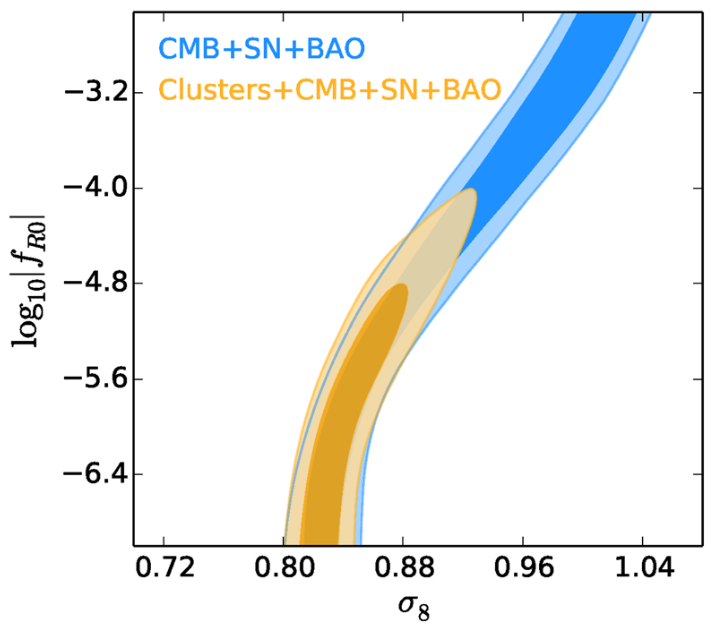
\includegraphics[height=.42\textwidth]{Cataneo_result.png} &
			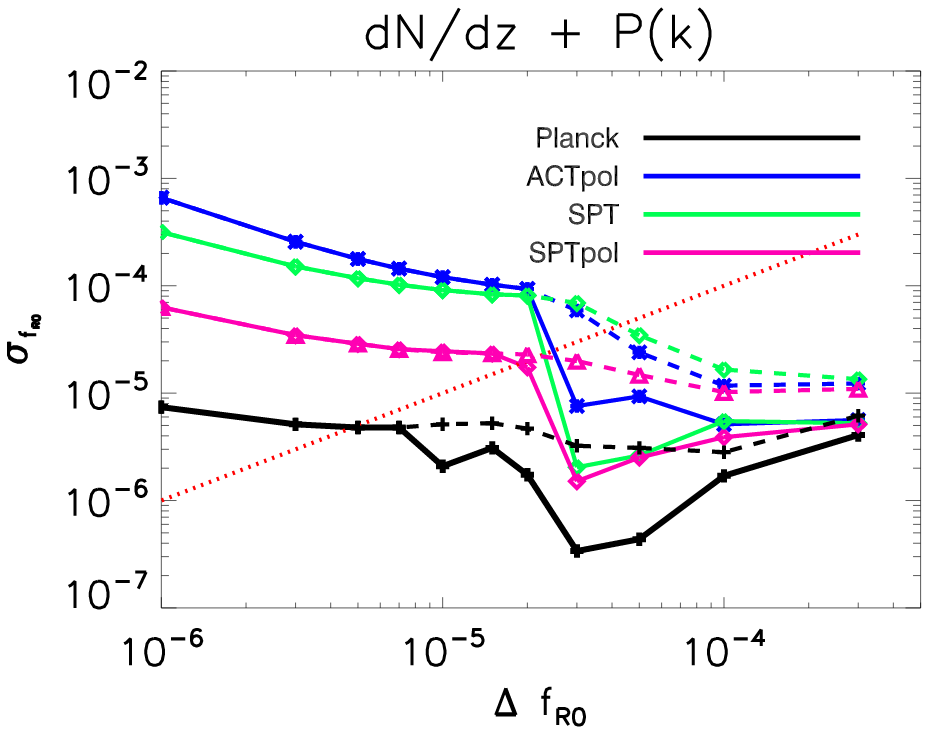
\includegraphics[height=.43\textwidth]{Mak_result.png} \\
		\end{tabular}
	\end{figure}
	\end{typewriter}
\end{frame}

% Final Slide/Thank You ------------------------------------------------

\fbckg{smile_cluster_2.png}
\begin{frame}[plain,noframenumbering]
	\pointedsl{darkred}{Questions ?}
\end{frame}

% Bibliography  ------------------------------------------------

%\fbckg{white.jpg} % Slide background image
%\begin{frame}[plain,noframenumbering]
%	\ftitle{Bibliography}
%	\begin{typewriter}
%		\begin{thebibliography}{10}
%			\bibitem{bhattacharya2011mass} Bhattacharya, S. et al.  ApJ 732.2 2011
%		\end{thebibliography}
%	\end{typewriter}
%\end{frame}

% Appendix ------------------------------------------------

%----------------------------------------------------------------------------------------

\end{document}

% Content ------------------------------------------------
%\fbckg{white.jpg} % Slide background image
%\begin{frame}
%	\begin{typewriter}
%	%{\LARGE Content}
%	\ftitle{Content}
%	\vspace{2em}
%	\begin{enumerate}
%		\item Introduction
%		\item Data
%		\item Methods
%		\item Results
%		\item Conclusion
%	\end{enumerate}
%	\end{typewriter}
%\end{frame}
